\newpage
\section{Pre-amplifier test}
This section will test all requirements related to the \gls{preamp}. 


\subsection{\autoref{req:preamp1}}
According to \autoref{req:preamp1}, a test was made to ensure that the \gls{preamp} does not change the signal amplitude more than $\pm$\SI{1}{\decibel} between 20 Hz and 20 kHz. A test was made and is descried in \autoref{app:preamp_frequency_response} and the result is seen in \autoref{fig:tests:appendix:amplitude}.

\begin{figure}[htbp!]
	\centering
		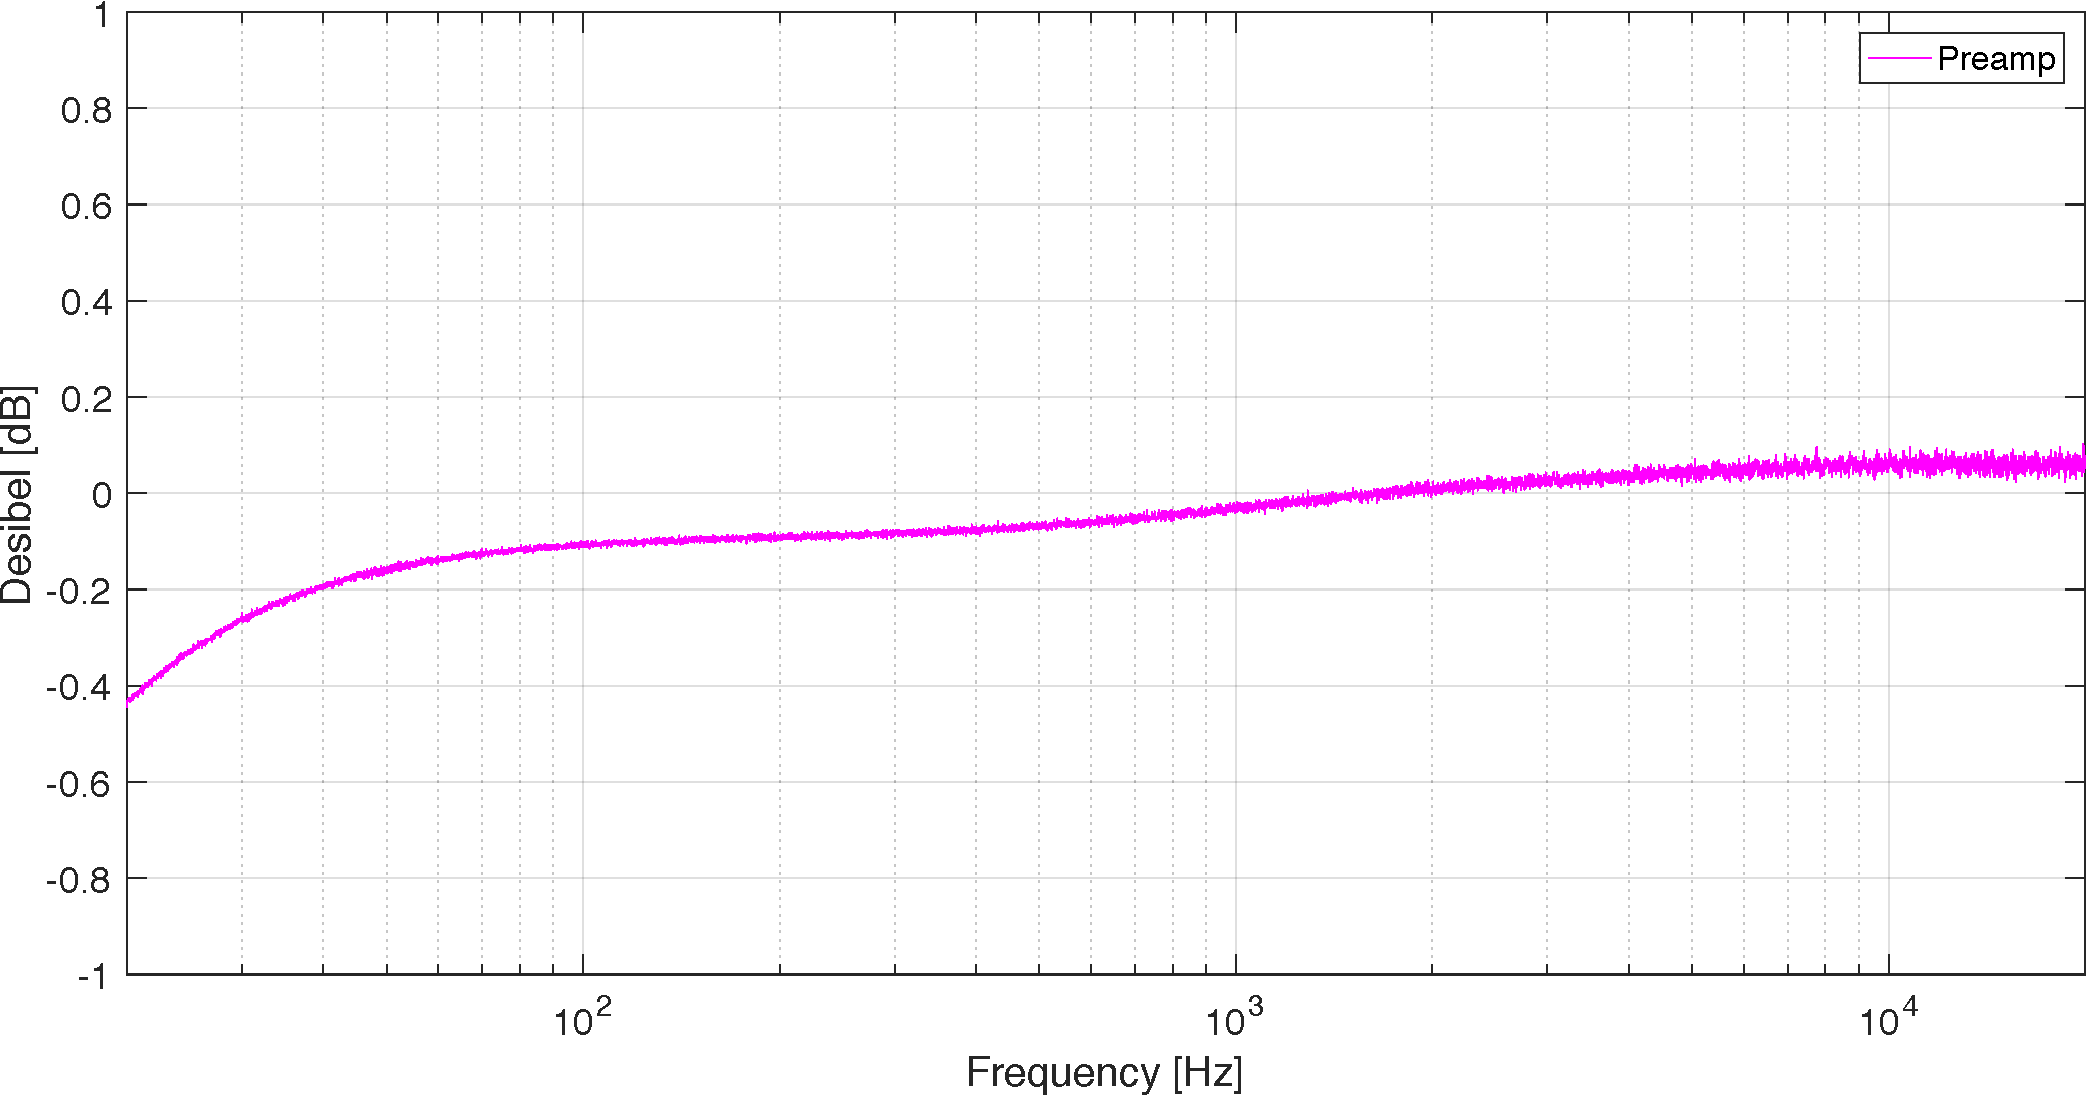
\includegraphics[width=1\textwidth]{preamp_frequency_responce.pdf}
		\caption{Measurement of the frequency response of the \gls{preamp}.}
		\label{fig:tests:appendix:amplitude}
\end{figure}

The amplitude is within $\pm$\SI{1}{\decibel} so \autoref{req:preamp1} is approved.


\subsection{\autoref{req:preamp2}}
According to \autoref{req:preamp2} the input impedance of  the \gls{preamp} must be at least 10 times the output impedance of the guitar. The requirement is assumed approved since the input impedance of an \gls{opamp} is normally between $10^5$ to $10^{12}$ $\Omega$, without a feedback loop. \autoref{eq:preamp_result} is therefore assumed correct and therefore the input impedance of the \gls{preamp} is \SI{1}{\mega\ohm}.
%According to \autoref{req:preamp2}, a test was made to ensure that the \gls{preamp} have an input impedance 10 times higher than the highest output impedance of the guitar. According to \autoref{app:output_impedance} and the requirements the \gls{preamp} shall have an input impedance of at least \SI{730.8}{\kilo\ohm}. To ensure that the input impedance is more than \SI{730.8}{\mega\ohm}. The input impedance of the \gls{opamp} was measured, and the result is to \SI{9.18}{\mega\ohm} according to \autoref{app:opamp_impedance}. Applying the input impedance to the following \autoref{eq:tests:preamp_result}, where $A$ is at least \SI{70}{\decibel}, according to \citep{TS464}.  
%
%\begin{equation}\label{eq:tests:preamp_result}
%        Z_{In_{G1}} = R_{Bias} \parallel ((Z_i + Z_{i \beta}) \cdot (1+\beta \cdot A)) \simeq R_{Bias}
%        \addunit{\si{\ohm}}
%    \end{equation}
%
%where the value from \autoref{label_Pre-amplifier} is applied as following \autoref{eq:tests:preamp_result_value}.



%
%\begin{subequations}\label{eq:tests:preamp_result_value}
%\begin{equation}
%        Z_{In_{G1}} = \SI{1}{\mega\ohm} \parallel ((\SI{9.18}{\mega\ohm} + 2550 \ohm) \cdot (1+ 0.5 \cdot 3162)) \simeq R_{Bias}
%        \addunit{\si{\ohm}}
%    \end{equation}
%\centering
%$\Updownarrow$
%\begin{equation}
%        Z_{In_{G1}} = \SI{1}{\mega\ohm} \parallel \SI{14.53}{\giga\ohm}  \simeq R_{Bias}
%        \addunit{\si{\ohm}}
%    \end{equation}
%    $\Updownarrow$
%\begin{equation}
%        \SI{999.9}{\kilo\ohm} = \SI{1}{\mega\ohm} \parallel \SI{14.53}{\giga\ohm} 
%        \addunit{\si{\ohm}}
%    \end{equation}
% \end{subequations}
%
%The calculated input impedance is higher than the required input impedance, so \autoref{req:preamp2} is approved.

\subsection{\autoref{req:preamp3}}
According to \autoref{req:preamp3} the output impedance of the preamp must be one tenth of the input impedance of the \gls{dsp}. The requirement is approved since the output impedance of an \gls{opamp} is normally between \SI{50}{\ohm} to \SI{200}{\ohm}, without a feedback loop. \autoref{eq:preamp_zout_out} is therefore assumed correct and thus the requirement is fulfilled.  

\subsection{\autoref{req:preamp4}}
The \gls{preamp} is designed to be supplied by a 5 to 9 voltage supply, and the \gls{preamp} will be supplied from a \SI{9}{\volt} battery. The \autoref{req:preamp4} is therefore approved.

\subsection{\autoref{req:preamp5} and \autoref{req:preamp6}}
According to \autoref{req:preamp6}, a test was made to ensure that the \gls{preamp} \gls{pcb} including cable mound fits into the jack connector house. \autoref{fig:tests:preamp_pcb} shows the \gls{pcb} mounded on the jack connector and the cable is mounted on the \gls{preamp}. 

 

\autoref{fig:tests:preamp_jack} shows the \gls{preamp} \gls{pcb} mounted inside the jack connector house.

\begin{figure}[htbp]
\centering
\begin{subfigure}[htbp]{0.35\textwidth}
		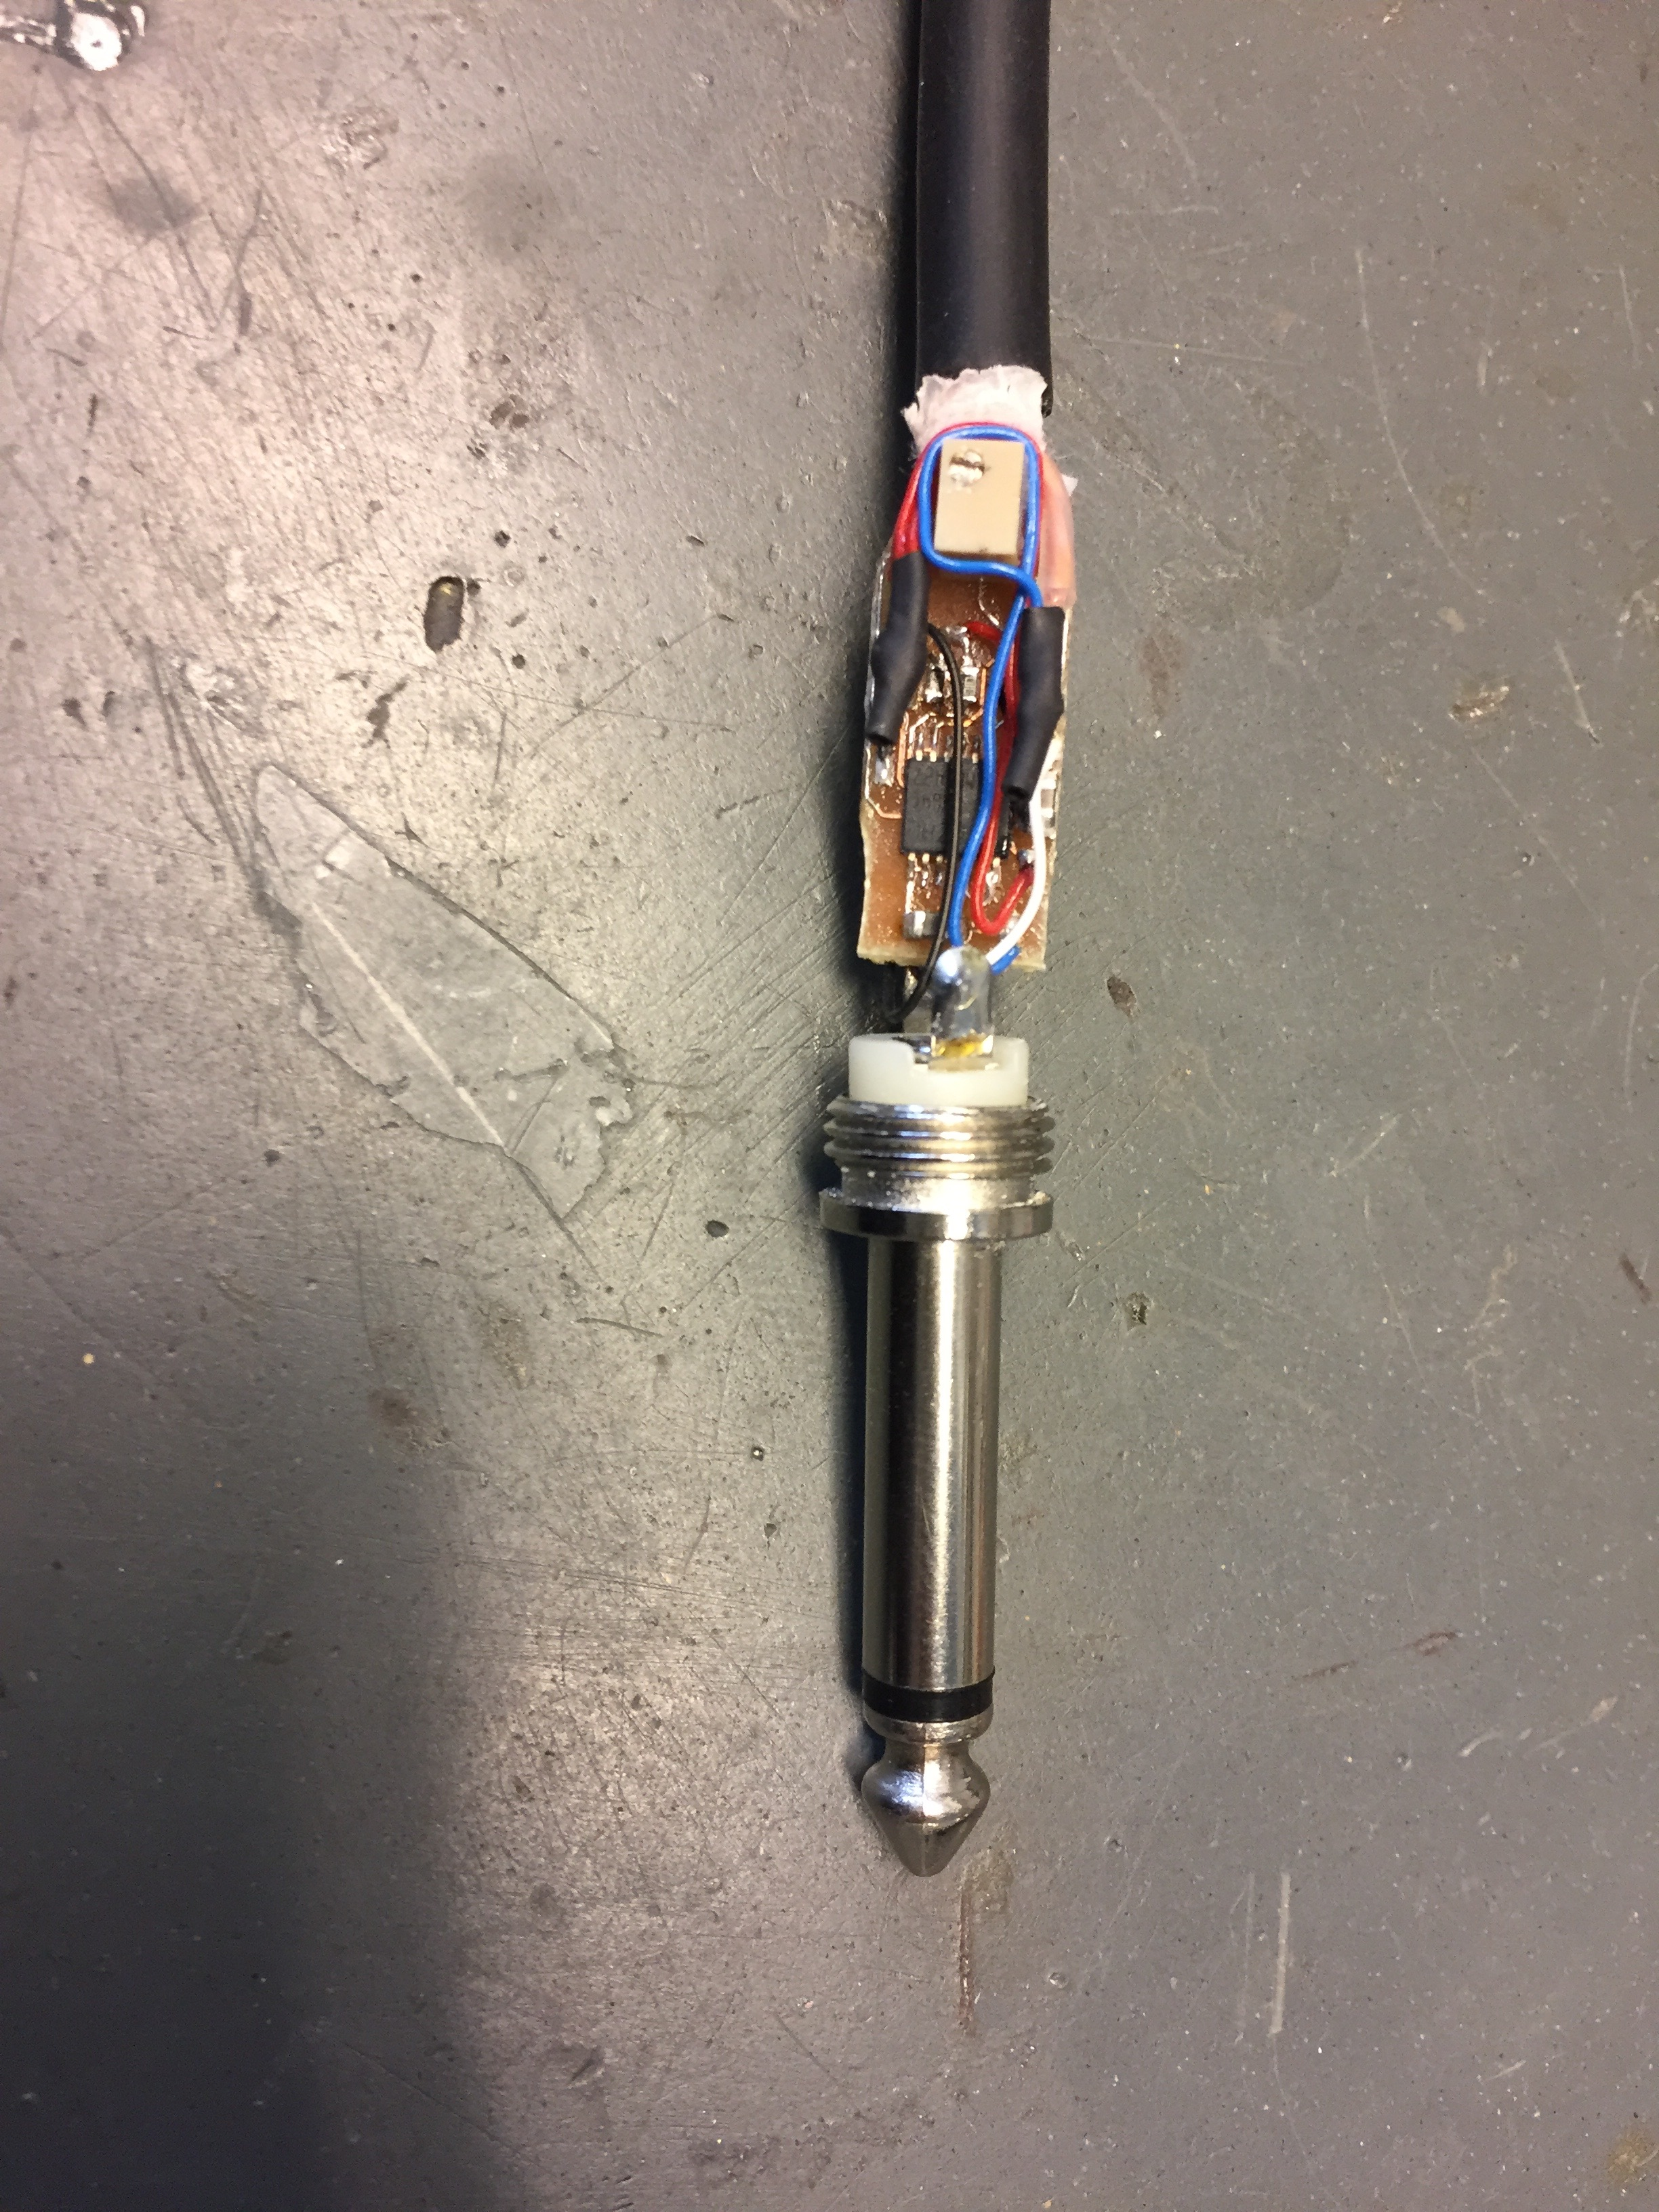
\includegraphics[width=\textwidth, angle=90]{preamp_pcb.jpg}
		\caption{The picture shows the mounted \gls{preamp} \gls{pcb} soldered to the jack connector}
		\label{fig:tests:preamp_pcb}
\end{subfigure}
 \qquad \qquad \qquad
\begin{subfigure}[htbp]{0.35\textwidth}
		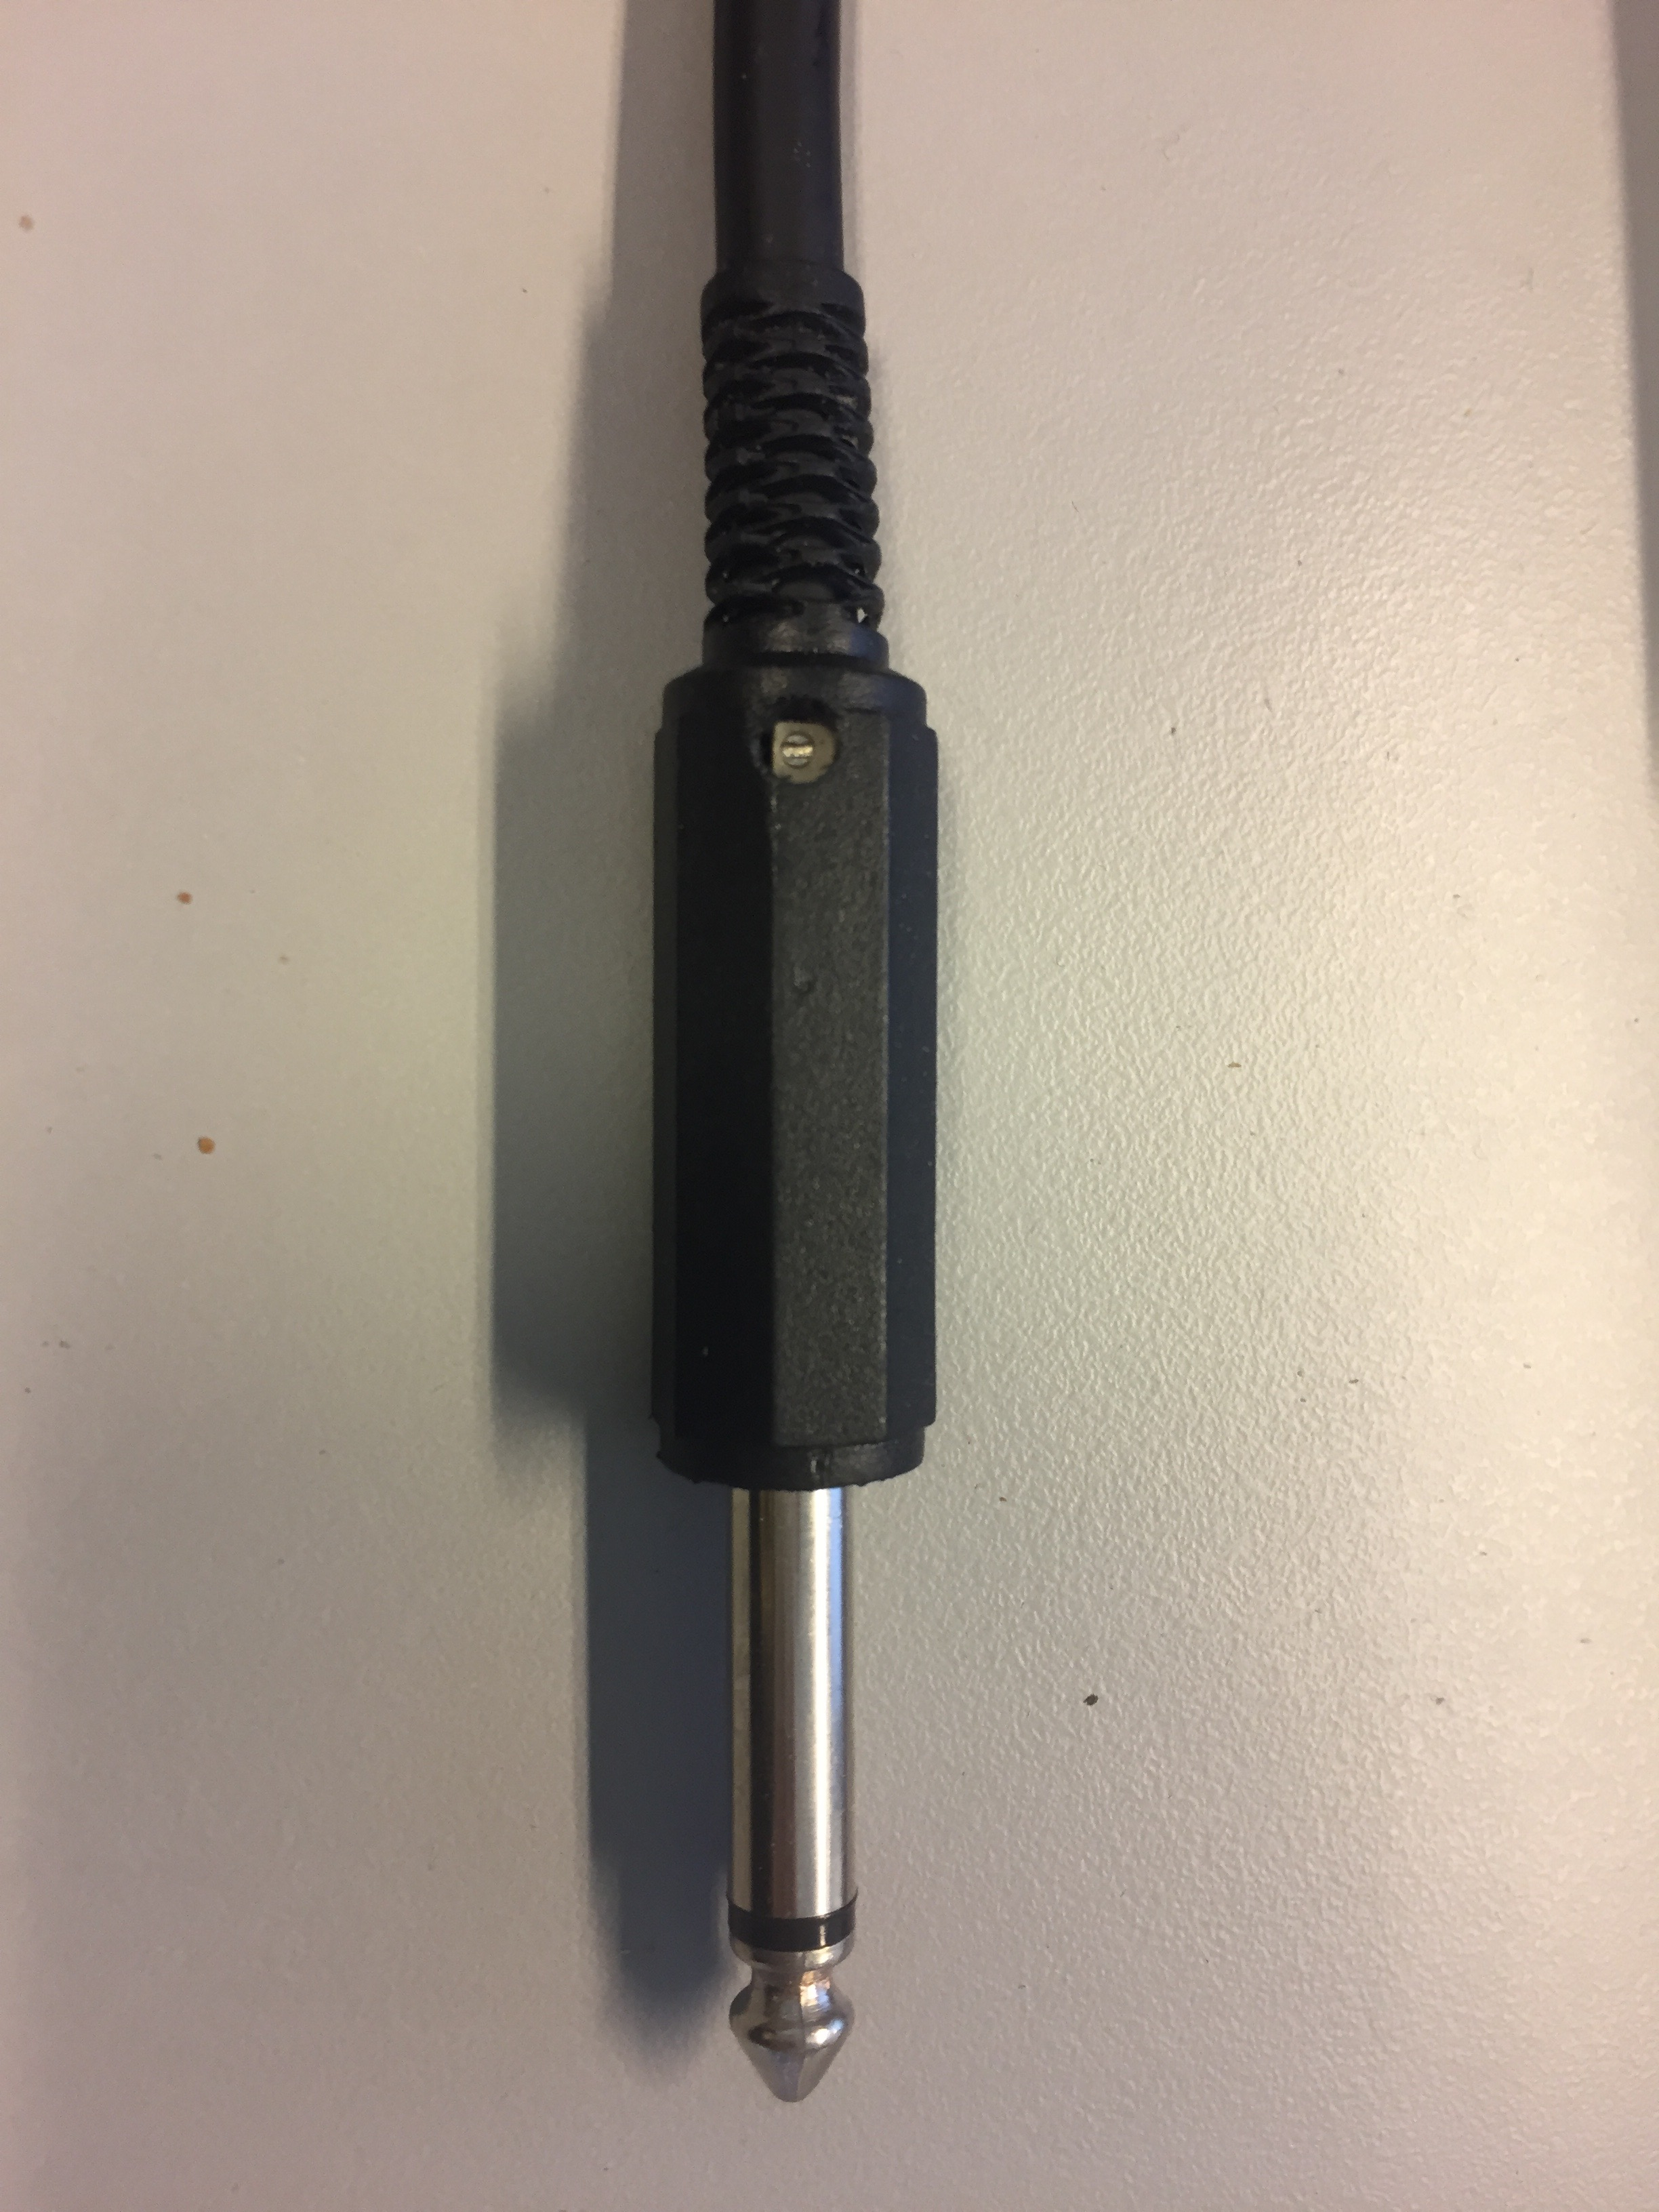
\includegraphics[width=\textwidth, angle=90]{preamp_jack.jpg}
		\caption{The picture shows the mounted \gls{preamp} \gls{pcb} inside the jack house.}
		\label{fig:tests:preamp_jack}
\end{subfigure} 
\caption{The \gls{preamp}}
\end{figure}

The \gls{preamp} \gls{pcb} fits inside the jack house, so \autoref{req:preamp5} and \autoref{req:preamp6} is approved.




\subsection{Test review of the \gls{preamp}}
In this subsection, a short review will be shown of the \gls{preamp} test.

\begin{table}[H]
\centering
\caption{Recap of the requirements fulfilments for the \gls{preamp} test}
\label{test_of_preamp_table}
\begin{tabular}{|l|l|}
\hline
\rowcolor[HTML]{9B9B9B} 
\textbf{Requirement} & \textbf{Fulfilment State} \\ \hline
\textbf{\ref{req:preamp1}}    & \cmark                     \\ \hline
\textbf{\ref{req:preamp2}}    & \cmark                     \\ \hline
\textbf{\ref{req:preamp3}}    & \cmark                     \\ \hline
\textbf{\ref{req:preamp4}}    & \cmark                      \\ \hline
\textbf{\ref{req:preamp5}}    & \cmark                     \\ \hline
\textbf{\ref{req:preamp6}}    & \cmark                     \\ \hline
\end{tabular}
\end{table}

